\chapter{发育遗传学与形态演化}\label{ch:b3:developmental-genetics}

果蝇的卵长半毫米，受精后的三小时内，
在其六千个细胞核之间尚未形成任何细胞膜之前，
它便已决定哪一端为头、哪一端为尾，
十四个体节各自的位置，以及其中哪些将长出腿、翅或触角。
它依靠几十个基因完成这一切，
这些基因以层层细化的条纹依次开启，每条条纹
由前一级条纹产物的浓度读取信息。1980 年，
海德堡的两位年轻科学家筛选了数千只突变果蝇，
寻找身体部分缺失或重复的幼虫，发现了整个
层级：有的基因缺失会使一段体节消失，有的基因
缺失会使每隔一个体节消失，有的基因缺失则使每个体节
前后颠倒。同年的一项工作针对一个基因：该基因能使果蝇的第三体节
变成第二体节的拷贝，使其长出四个翅膀，与其祖先相同——
这一发现揭示了一组主控基因，
这些基因在小鼠与人的染色体上排列顺序相同，
且功能相同。本章讨论胚胎如何计算自身的几何结构，
几百个调控基因如何构建每一种动物的身体，
以及它们何时、何处发挥作用的改变如何产生了
动物形态的多样性。

\section{果蝇的坐标}

\begin{definition}[体节划分层级]\label{def:b3:developmental-genetics:hierarchy}
\index{母体效应基因}\index{裂隙基因}\index{成对规则基因}\index{体节极性基因}\index{合胞体胚盘}
\emph{Drosophila} 胚胎在最初十三次核分裂期间，
以\emph{合胞体胚盘}的形式发育，这是一个单细胞，其细胞核
共享同一细胞质，蛋白质可从其
合成之处自由扩散。母体细胞形成的四个梯度确定了各轴向：
\emph{bicoid} mRNA 锚定于前极，其蛋白质
向后扩散，形成一条从头到尾的指数梯度；
\emph{nanos} mRNA 位于后极，形成镜像梯度；
\emph{hunchback} 与 \emph{caudal} 的 mRNA 分布均匀，但 Bicoid
蛋白抑制 \emph{caudal} 的翻译，Nanos 抑制
\emph{hunchback}，因此二者的蛋白质也形成梯度。这些
这些\emph{母体效应}产物，其突变表型取决于
母体的基因型而非胚胎的基因型，开启\emph{裂隙基因}
（\emph{hunchback}、\emph{Krüppel}、\emph{knirps}、\emph{giant}）以
宽带的形式出现，每条带响应一定范围的 Bicoid 浓度，
并抑制相邻的带；裂隙蛋白共同开启
\emph{成对规则基因}（\emph{even-skipped}、\emph{fushi tarazu}、
\emph{hairy}），各形成七条交替条纹；成对规则蛋白
开启\emph{体节极性基因}（\emph{engrailed}、
\emph{wingless}、\emph{hedgehog}）形成十四条条纹，每个体节一条，
它们确定每个体节的前后界，并在细胞形成后
由细胞间的信号传递维持。三小时内，四个层级，由单一梯度
产生十四个体节，突变基因的命名记录
了这次筛选：\emph{hunchback} 缺失胸部，\emph{Krüppel}（“残缺”）
缺失中部，\emph{fushi tarazu}（“体节不足”）使每隔一个
体节缺失，\emph{hedgehog} 体表则长满刚毛。
\end{definition}

\begin{omfigure}
\begin{tikzpicture}[every node/.style={font=\scriptsize}, >=stealth]
  \foreach \y/\lab/\n in {0/{母体效应：Bicoid 梯度}/1, -1.3/{裂隙基因：4 条宽带}/2, -2.6/{成对规则基因：7 条条纹}/3, -3.9/{体节极性基因：14 条条纹}/4} {
    \draw[thick, gray!60] (0,\y) ellipse (3.6 and 0.5);
    \node[left, align=right] at (-3.8,\y) {\lab};
  }
  % bicoid gradient shading
  \begin{scope}
    \clip (0,0) ellipse (3.6 and 0.5);
    \shade[left color=omDef!80, right color=omDef!2] (-3.6,-0.5) rectangle (3.6,0.5);
  \end{scope}
  \node[right, font=\tiny] at (3.7,0) {前端高};
  % gap bands
  \begin{scope}
    \clip (0,-1.3) ellipse (3.6 and 0.5);
    \fill[omDef!50] (-3.4,-1.8) rectangle (-1.6,-0.8); \fill[omThm!40] (-1.4,-1.8) rectangle (0.2,-0.8); \fill[omMeth!40] (0.4,-1.8) rectangle (1.7,-0.8); \fill[omProp!45] (1.9,-1.8) rectangle (3.4,-0.8);
  \end{scope}
  \node[font=\tiny] at (-2.5,-1.3) {裂隙 \emph{hb}}; \node[font=\tiny] at (-0.6,-1.3) {裂隙 \emph{Kr}}; \node[font=\tiny] at (1.05,-1.3) {裂隙 \emph{kni}}; \node[font=\tiny] at (2.65,-1.3) {裂隙 \emph{gt}};
  % pair-rule stripes
  \begin{scope}
    \clip (0,-2.6) ellipse (3.6 and 0.5);
    \foreach \i in {0,...,6} { \fill[omThm!50] ({-3.1+\i*0.9},-3.1) rectangle ({-2.75+\i*0.9},-2.1); }
  \end{scope}
  \node[right, font=\tiny] at (3.7,-2.6) {\emph{eve}，隔一个体节};
  % segment polarity stripes
  \begin{scope}
    \clip (0,-3.9) ellipse (3.6 and 0.5);
    \foreach \i in {0,...,13} { \fill[omProp!60] ({-3.25+\i*0.47},-4.4) rectangle ({-3.1+\i*0.47},-3.4); }
  \end{scope}
  \node[right, font=\tiny] at (3.7,-3.9) {\emph{en}：每个体节一条};
  \foreach \y in {-0.55,-1.85,-3.15} { \draw[->, thick] (0,\y) -- (0,\y-0.2); }
  \node[below, align=center, font=\tiny] at (0,-4.5) {每一层读取上一层的浓度；\\三小时内，由单一梯度产生十四个体节};
\end{tikzpicture}

{\small 体节划分层级。母体梯度被读取为
四条\omterm{def:b3:developmental-genetics:hierarchy}{裂隙基因}带；裂隙蛋白共同形成七条
成对规则条纹；这些再形成十四条体节极性条纹。每
一条条纹都是浓度越过阈值之处所划定的边界。}
\end{omfigure}

\begin{theorem}[由合成、扩散与降解形成的形态发生素梯度]\label{thm:b3:developmental-genetics:gradient}
\index{形态发生素}\index{位置信息}\index{法国国旗模型}\index{衰减长度}
在组织的一端，一种蛋白质以速率 $J$（按单位面积计）产生，
以扩散系数 $D$ 扩散，以速率常数 $k$ 降解，
最终达到稳态，其沿轴线 $x$ 的浓度
满足下式：
\[
D\,\frac{\mathrm{d}^{2}c}{\mathrm{d}x^{2}} - k\,c = 0,
\qquad c(x) = c_{0}\,\mathrm{e}^{-x/\lambda}, \qquad \lambda = \sqrt{D/k},
\quad c_{0} = \frac{J}{\sqrt{Dk}} .
\]
\emph{\omterm{thm:b3:developmental-genetics:gradient}{衰减长度}} $\lambda$ 决定梯度的作用范围；细胞
通过比较 $c$ 与阈值来读取自身位置——
即沃尔珀特（1969）提出的\emph{法国国旗}模型：高于 $T_{1}$ 为蓝色，介于
$T_{1}$ 与 $T_{2}$ 之间为白色，低于此值为红色——对阈值 $T$ 而言，边界
位于 $x_{T} = \lambda\ln(c_{0}/T)$ 处。两点推论：源的强度加倍
使每个边界都后移相同的 $\lambda\ln 2$，同时
读取浓度的相对误差 $\delta c/c$ 即是
位置误差 $\delta x = \lambda\,\delta c/c$，因此梯度只有
将边界定位到一个细胞之内，仅当细胞读取浓度的误差
在百分之几以内。Bicoid 的\omterm{thm:b3:developmental-genetics:gradient}{衰减长度} $\lambda \approx \qty{100}{\micro m}$，位于
长 \qty{500}{\micro m} 的卵内：梯度跨越的倍数为 $\mathrm{e}^{5}
\approx 150$，而 \emph{hunchback} 的边界位于卵的中部，此处
Bicoid 的浓度已降至峰值的约十二分之一。
\end{theorem}
\begin{proof}
对 $x$ 与 $x + \mathrm{d}x$ 之间的薄层应用守恒：净
扩散流入量 $D\,\partial^{2}c/\partial x^{2}$ 与
稳态下的降解量 $kc$ 相平衡，得到该方程；其解
在 $x \to \infty$ 时有界，为衰减指数函数，满足
$\lambda^{2} = D/k$。源项：$x = 0$ 处的扩散通量 $-D\,
c'(0) = Dc_{0}/\lambda$ 等于 $J$，故 $c_{0} = J\lambda/D =
J/\sqrt{Dk}$。阈值：由 $c_{0}\mathrm{e}^{-x_{T}/\lambda} = T$ 得
$x_{T}$；$c_{0}$ 加倍则 $\lambda\ln 2$ 加到每个 $x_{T}$ 上，
与 $T$ 无关。误差：对 $x_{T} = \lambda\ln(c_{0}/c)$ 求导，
$\delta x = -\lambda\,\delta c/c$。稳态是在
时间尺度 $1/k$ 上达到的，对 Bicoid 而言，该尺度（\qty{50}{min}）与
可用的两小时相当，因此梯度在尚未稳定时即已被读取。
\end{proof}

\begin{omfigure}
\begin{tikzpicture}
\begin{axis}[
  width=0.7\linewidth, height=5.6cm,
  axis x line=bottom, axis y line=left,
  xmin=0, xmax=500, ymin=0, ymax=1.05,
  xlabel={距前极的距离（\unit{\micro m}）}, ylabel={Bicoid，相对值},
  xlabel style={font=\small, at={(axis description cs:0.5,-0.12)}, anchor=north}, ylabel style={font=\small},
  tick label style={font=\small}, xtick={0,100,250,400,500}, ytick={0.08,0.3,0.6,1},
  yticklabels={0.08,0.3,0.6,1},
  clip=false,
]
\fill[omDef!15] (axis cs:0,0) rectangle (axis cs:120,1.05);
\fill[gray!8] (axis cs:120,0) rectangle (axis cs:250,1.05);
\fill[omThm!12] (axis cs:250,0) rectangle (axis cs:500,1.05);
\addplot[very thick, omDef, domain=0:500, samples=100] {exp(-x/100)};
\addplot[thick, omDef!50, dashed, domain=66:500, samples=100] {2*exp(-x/100)};
\draw[dashed, gray] (axis cs:0,0.3) -- (axis cs:120,0.3) -- (axis cs:120,0);
\draw[dashed, gray] (axis cs:0,0.08) -- (axis cs:250,0.08) -- (axis cs:250,0);
\node[font=\scriptsize, anchor=south] at (axis cs:60,1.0) {头};
\node[font=\scriptsize, anchor=south] at (axis cs:185,1.0) {胸};
\node[font=\scriptsize, anchor=south] at (axis cs:375,1.0) {腹};
\node[font=\scriptsize, omDef, anchor=west] at (axis cs:255,0.35) {$c = c_{0}\,\mathrm{e}^{-x/\lambda}$, $\lambda = \qty{100}{\micro m}$};
\node[font=\scriptsize, omDef!70!black, anchor=west, align=left] at (axis cs:255,0.62) {虚线：源加倍——\\每条边界移动 $\lambda\ln 2 = \qty{69}{\micro m}$};
\node[font=\scriptsize, gray, anchor=north east] at (axis cs:118,0.29) {$T_{1}$};
\node[font=\scriptsize, gray, anchor=south west] at (axis cs:300,0.09) {$T_{2}$：\emph{hunchback} 关闭};
\end{axis}
\end{tikzpicture}

{\small 由指数函数画出的“法国国旗”。同一梯度上的阈值
划分卵的各个区域；较强的源会使所有
边界向后移动相同的距离，这正是
额外携带 \emph{bicoid} 拷贝的母体所产胚胎所表现出的情形。}
\end{omfigure}

\begin{proof}[证据]
纽斯莱因-福尔哈德和维绍斯（1980）用\omterm{met:b3:cancer-biology:ames}{诱变剂}喂食果蝇，培育
子代至纯合，并在显微镜下观察部分
\num{27000} 只死亡幼虫的角质层，以查找缺失或重复的
图式：约一百二十个基因，按其表型归入
\omterm{def:b3:developmental-genetics:hierarchy}{裂隙基因}、\omterm{def:b3:developmental-genetics:hierarchy}{成对规则基因}和\omterm{def:b3:developmental-genetics:hierarchy}{体节极性基因}三类——一种层级结构，
在任何分子被认识之前即已可见。德里弗和纽斯莱因-福尔哈德
（1988）对胚胎进行 Bicoid 蛋白染色，看到自前极起的
指数梯度；母体携带一、二、
四或六个该基因拷贝的母体所产胚胎的梯度高度成比例，
头部褶与 \emph{hunchback} 边界均随剂量
向后移动，正如阈值模型所预测，移动量大致为
每次加倍所需的 $\lambda\ln 2$。注入 \emph{bicoid} mRNA
至卵的中部，便在该处形成一个头部。
\end{proof}

\begin{omfigure}
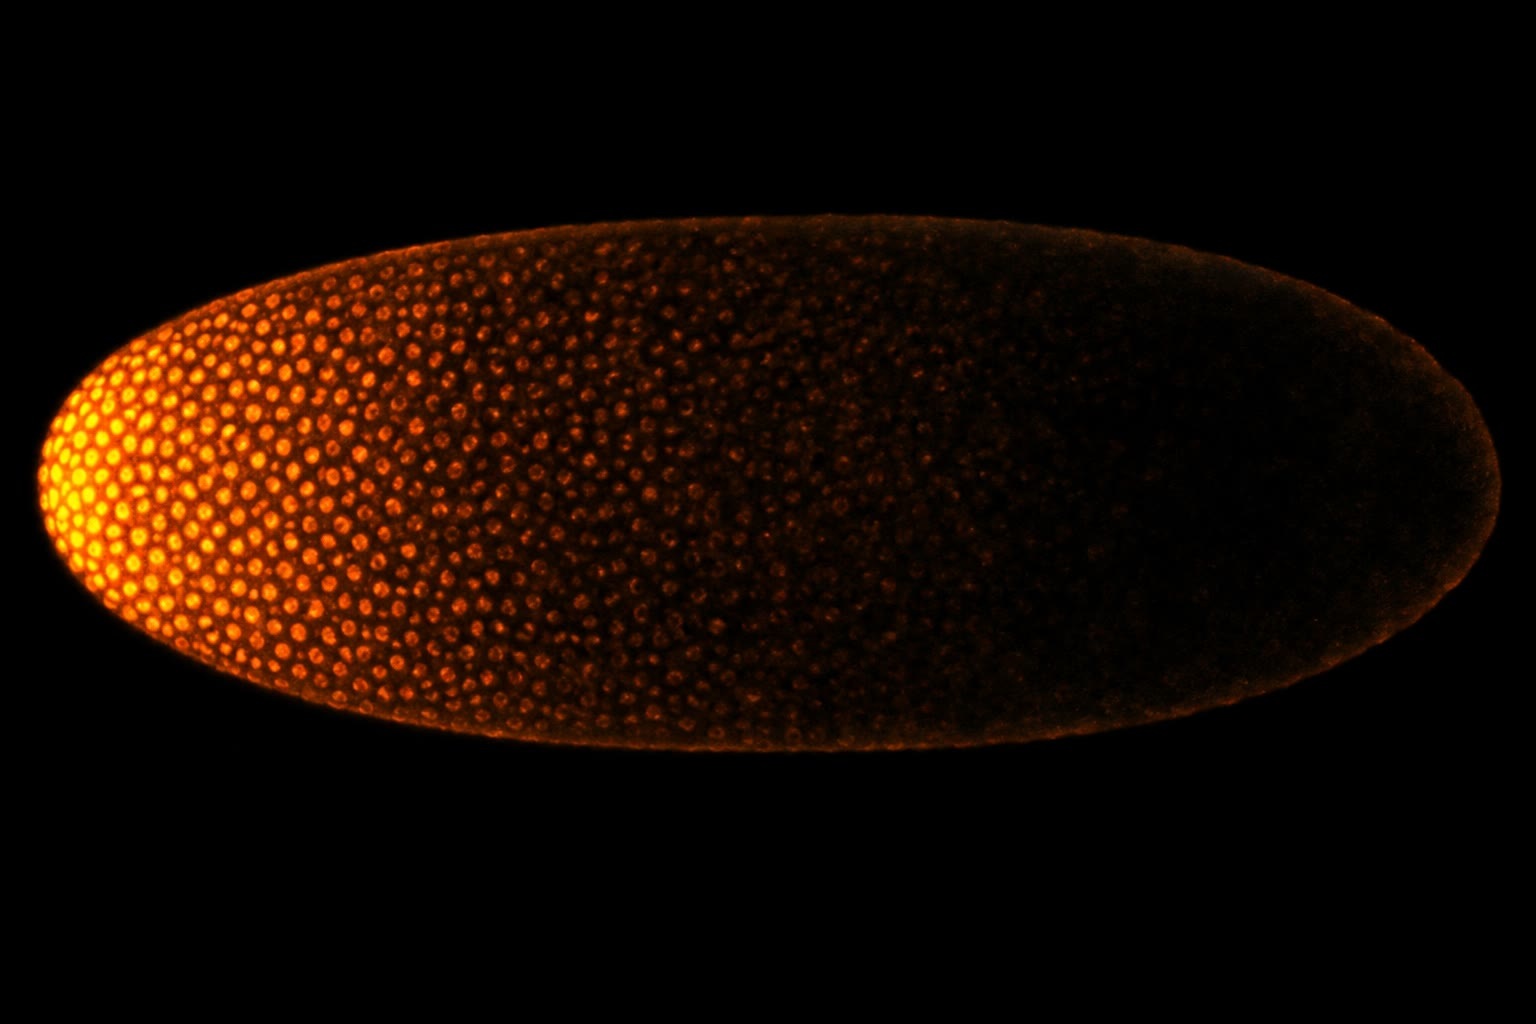
\includegraphics[width=0.46\linewidth]{images/book5/ai/b5-23-bicoid-gradient.jpg}\hspace{0.04\linewidth}
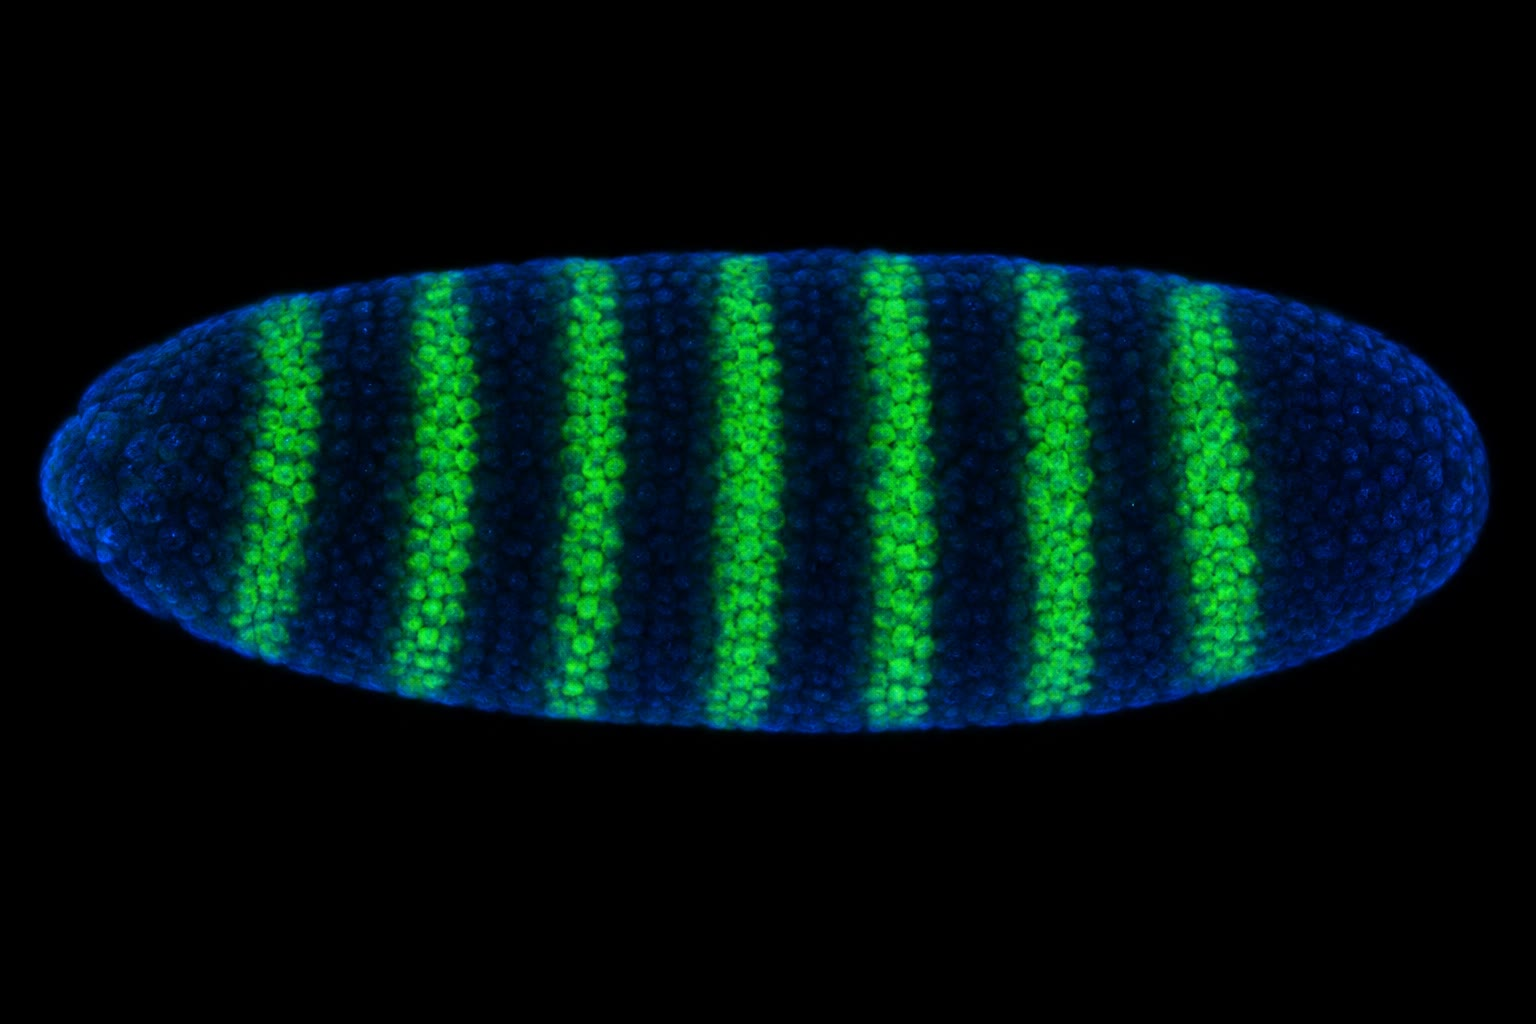
\includegraphics[width=0.46\linewidth]{images/book5/ai/b5-23-embryo-stripes.jpg}

{\small 左：合胞体胚经 Bicoid 蛋白染色，亮度
在前极最强，并向后端呈指数减弱。
右：一小时后的胚胎经成对规则蛋白染色，显示
七条条纹，由\omterm{def:b3:developmental-genetics:hierarchy}{裂隙基因}的条带勾勒而成。}
\end{omfigure}

\section{身份：Hox 基因}

\begin{definition}[同源异型基因与共线性]\label{def:b3:developmental-genetics:hox}
\index{同源异型突变}\index{Hox 基因}\index{共线性}\index{同源框}\index{Hox 密码}
\emph{同源异型}突变使一个身体部分变成另一个：
贝特森（1894）提出的术语，指那些“以一个
系列中的一员替换另一员。”在果蝇中，\emph{Antennapedia}
显性突变体在应长触角的地方长出腿；\emph{bithorax}
突变体（路易斯，1978）使第三胸节变成了第二胸节的
复制品，使平衡棒变成了第二对
翅。负责的八个基因，即 \emph{Hox 基因}，分布于
同一条染色体上的两个簇中，路易斯注意到，它们沿 DNA 的
排列顺序与其所控制的体节沿身体的排列顺序相一致
——\emph{共线性}，至今尚未完全解释。每个基因都编码一种
转录因子，它们具有相同的 60 个氨基酸的 DNA 结合
\emph{同源框}结构域（麦金尼斯、格林，1984），该结构域随后
被发现存在于所有动物中：小鼠和人类各携带四个簇，每簇十三个基因，
各自同样具有共线性，以嵌套的结构域沿
体轴表达，簇中靠后的基因位于更后方。细胞沿体轴的
身份由其所表达的 Hox 基因组合给出，即
\emph{Hox 密码}；后位基因压制前位基因（后位优势），
因此失去一个后位基因，会使该体节
采用其前方那一个的身份。Hox 基因并不构建
体节，而是告诉已建成的体节它是哪一种，
通过开启一组下游基因，这些基因适于形成
腿、翅、肋骨或腰椎。
\end{definition}

\begin{omfigure}
\begin{tikzpicture}[every node/.style={font=\scriptsize}, >=stealth]
  % fly cluster
  \node[left] at (-0.3,2.2) {果蝇（\emph{Drosophila}），8 个基因};
  \foreach \i/\g/\c in {0/lab/omDef, 1/pb/omDef, 2/Dfd/omThm, 3/Scr/omThm, 4/Antp/omMeth, 5/Ubx/omMeth, 6/abd-A/omProp, 7/Abd-B/omProp} {
    \draw[thick, fill=\c!40] ({\i*1.1},1.9) rectangle ({\i*1.1+0.9},2.5); \node[font=\tiny] at ({\i*1.1+0.45},2.2) {\emph{\g}};
  }
  \node[left] at (-0.3,0.9) {小鼠 HoxB 簇，13 个中的 9 个};
  \foreach \i/\g/\c in {0/b1/omDef, 1/b2/omDef, 2/b3/omDef, 3/b4/omThm, 4/b5/omThm, 5/b6/omMeth, 6/b7/omMeth, 7/b8/omProp, 8/b9/omProp} {
    \draw[thick, fill=\c!40] ({\i*1.1},0.6) rectangle ({\i*1.1+0.9},1.2); \node[font=\tiny] at ({\i*1.1+0.45},0.9) {\emph{\g}};
  }
  \draw[->, thick] (0,1.55) -- (9.8,1.55); \node[above, font=\tiny] at (4.9,2.55) {沿 DNA 方向：3$'$ $\to$ 5$'$};
  \draw[->, thick] (0,0.2) -- (9.8,0.2); \node[below, font=\tiny] at (4.9,0.05) {沿身体由前 $\to$ 后};
  % body schematic
  \node[left] at (-0.3,-0.9) {表达于};
  \draw[thick, gray!70, rounded corners=6pt] (0,-1.3) rectangle (9.8,-0.5);
  \foreach \x/\t in {0.6/头, 2.6/颈, 4.4/胸, 6.6/腰, 8.6/{骶、尾}} { \node[font=\tiny] at (\x,-0.9) {\t}; }
  \draw[gray!70] (1.6,-1.3) -- (1.6,-0.5); \draw[gray!70] (3.5,-1.3) -- (3.5,-0.5); \draw[gray!70] (5.6,-1.3) -- (5.6,-0.5); \draw[gray!70] (7.6,-1.3) -- (7.6,-0.5);
  \node[below, align=center, font=\tiny] at (4.9,-1.4) {共线性：染色体上基因的顺序，即其结构域沿身体的排列顺序；\\同样的簇、同样的顺序，从果蝇到小鼠——\\继承自 6 亿年前的祖先};
\end{tikzpicture}

{\small 果蝇和小鼠中的 Hox 基因簇。基因沿 DNA 排列，
其顺序与两种动物中它们所决定的身体区段顺序一致，并且
同源基因可以通过序列加以区分：小鼠的 \emph{Hoxb6} 基因
明显就是果蝇的 \emph{Antennapedia}。}
\end{omfigure}

\begin{proof}[证据]
路易斯（1978 年）将 \emph{bithorax} 复合体作图，
发现它是一系列突变，每个突变使一个体节转变为其前方的体节，
这些突变在染色体上按身体顺序排列，并提出这些基因
沿体轴依次被激活。麦金尼斯及其同事（1984 年）
通过 \emph{Antennapedia} 与
\emph{Ultrabithorax} 之间的交叉杂交发现了\omterm{def:b3:developmental-genetics:hox}{同源框}，随后又在蛙和小鼠中得到确认；功能上的
等同性得到直接证明：小鼠的 \emph{Hoxb6} 基因在果蝇中表达，
产生 \emph{Antennapedia} 表型，即由触角变为腿
（20 世纪 90 年代）；缺失 \emph{Hoxc8} 的小鼠
第一腰椎多出一根肋骨，该体节获得了其前方体节的身份；
改变鸡和小鼠中的 Hox 表达边界，
会使前肢形成的位置移动，而天鹅颈的长度
则与同一边界的后移相对应。
\end{proof}

\begin{omfigure}
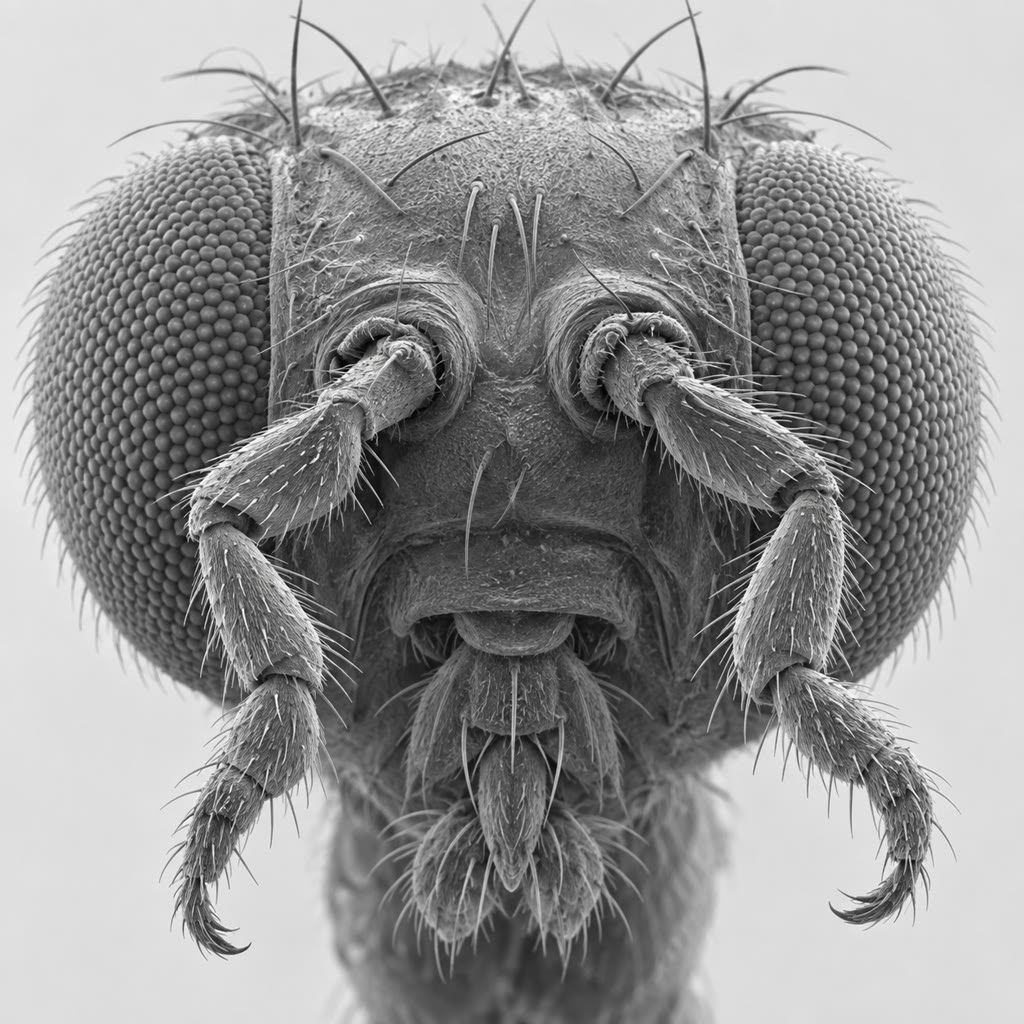
\includegraphics[width=0.34\linewidth]{images/book5/ai/b5-23-antennapedia-fly.jpg}\hspace{0.04\linewidth}
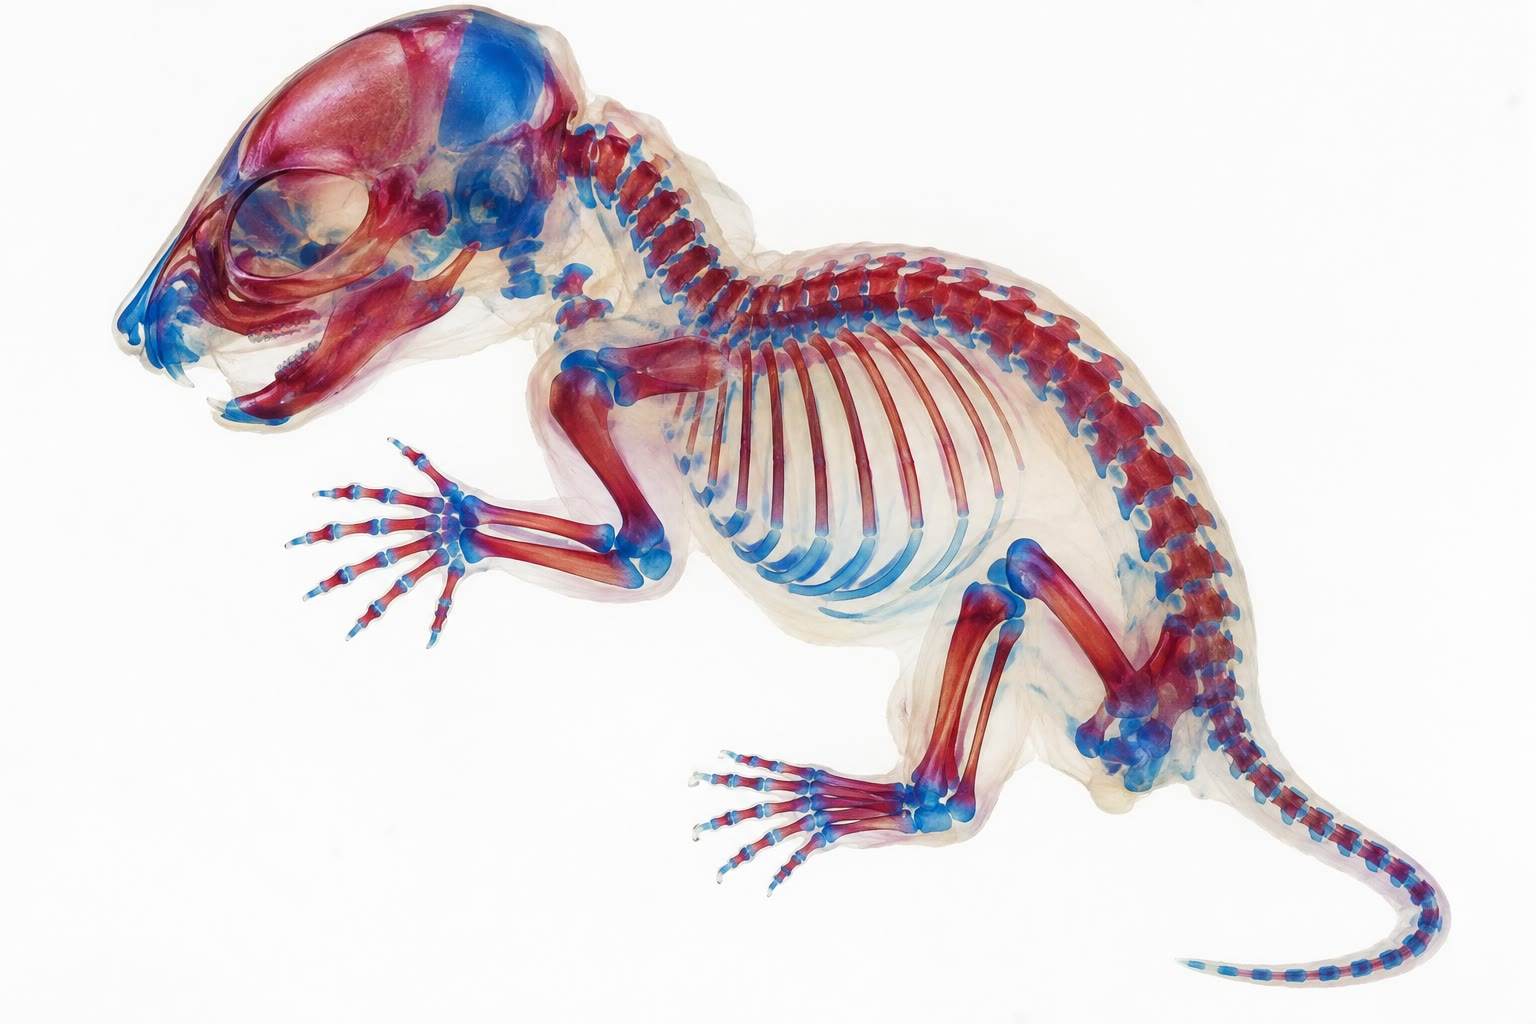
\includegraphics[width=0.5\linewidth]{images/book5/ai/b5-23-limb-skeleton-stain.jpg}

{\small 左：\emph{Antennapedia} 突变果蝇的头部，
本应是触角的位置长出一对腿——体节构造正确，
却被赋予了错误的身份。右：小鼠胚胎的骨骼，软骨
染蓝色，骨染红色，沿这些脊椎读取 Hox 密码。}
\end{omfigure}

\section{构建脊椎动物}

\begin{definition}[组织者与信号中心]\label{def:b3:developmental-genetics:organiser}
\index{组织者}\index{诱导}\index{Sonic hedgehog}\index{肢芽}\index{极性活性区}\index{顶端外胚层嵴}
脊椎动物胚胎从一开始就是细胞化的，因此其梯度由
分泌蛋白形成，而非合胞体的扩散形成，并且
同样少数几个家族承担全部功能：Wnt、Hedgehog、BMP 及其他 TGF-$\beta$
家族成员、FGF、Notch 和视黄酸。施佩曼与曼戈尔德（1924 年）
将蝾螈原肠胚背唇的一小块移植到另一胚胎的腹侧，
得到一个主要由宿主细胞构成、头尾俱全的第二胚胎：
该移植体即\emph{组织者}，诱导邻近细胞形成
神经系统和轴，其分子在七十年后被发现
是分泌性拮抗剂（Chordin、Noggin），它们阻断
BMP，而 BMP 缺失时外胚层便发育为神经组织——即默认命运。
\emph{神经管}随后在背腹方向上，由脊索和底板发出的 \emph{Sonic
hedgehog}（高浓度：运动神经元；低浓度：
\omterm{def:b3:nervous-systems:cells}{中间神经元}）进行模式化，与来自顶板的 BMP 相抗衡；\emph{肢芽}则由两个
中心决定：后缘的\emph{极性活性区}，
分泌 Shh（将其移植到前缘会使指发生镜像重复，
形成六指，拇指对拇指相接）；另一个是
尖端的\emph{顶端外胚层嵴}，分泌 FGF，维持下方细胞
持续分裂，并决定由近端到远端的顺序：
肱骨、前臂、手。移植、消融以及浸有蛋白质的珠子仍是主要手段；
其逻辑——局部来源、梯度、
阈值以及转录因子编码——都与果蝇相同。
\end{definition}

\begin{omfigure}
\begin{tikzpicture}[every node/.style={font=\scriptsize}, >=stealth]
  % limb bud
  \fill[omDef!12] (0,0) -- (0,3) .. controls (2.6,3.4) and (3.4,2.2) .. (3.4,1.5) .. controls (3.4,0.8) and (2.6,-0.4) .. (0,0) -- cycle;
  \draw[thick, omDef] (0,0) -- (0,3) .. controls (2.6,3.4) and (3.4,2.2) .. (3.4,1.5) .. controls (3.4,0.8) and (2.6,-0.4) .. (0,0);
  \draw[very thick, omMeth!70!black] (2.9,2.5) .. controls (3.45,1.9) and (3.45,1.1) .. (2.9,0.5);
  \node[right, align=left, omMeth!70!black, font=\tiny] at (3.5,1.5) {顶端外胚层嵴：\\FGF8；维持 \\生长区分裂；\\近端 $\to$ 远端};
  \begin{scope}
    \clip (0,0) -- (0,3) .. controls (2.6,3.4) and (3.4,2.2) .. (3.4,1.5) .. controls (3.4,0.8) and (2.6,-0.4) .. (0,0) -- cycle;
    \foreach \i/\op in {1/50, 2/38, 3/26, 4/14} { \draw[omThm!\op, thick] (0.6,0.5) circle ({0.45*\i}); }
  \end{scope}
  \fill[omThm!50] (0.6,0.5) ellipse (0.5 and 0.35); \node[anchor=north, align=center, omThm, font=\tiny] at (0.9,-0.2) {ZPA：Sonic hedgehog，\\后 $\to$ 前};
  \node[left, font=\tiny] at (-0.05,2.6) {前部}; \node[left, font=\tiny] at (-0.05,0.4) {后部};
  \node[left, font=\tiny] at (-0.05,1.5) {体壁};
  \draw[->, thick] (0.3,1.5) -- (3.0,1.5); \node[above, font=\tiny] at (1.75,1.55) {肱骨、前臂、指};
  % right: digit code
  \node[right, align=left] at (7.2,2.6) {指的身份取决于 Shh 暴露：\\拇指（第 1 指）：无；\\第 2--3 指：梯度；\\第 4--5 指：来自表达 Shh 的细胞};
  \node[right, align=left] at (7.2,1.0) {在前部移植第二个 ZPA：\\镜像重复，4-3-2-2-3-4；\\Shh 蛋白珠同样如此};
  \node[right, align=left, gray] at (7.2,-0.2) {同一分子也对神经管 \\（高浓度处为运动神经元）及肠道进行模式划分};
\end{tikzpicture}

{\small \omterm{def:b3:developmental-genetics:organiser}{肢芽}的两个信号中心。来自后缘的 Sonic hedgehog
告诉细胞将发育成哪一指；来自尖端的 FGF
告诉细胞它们在肢体上的远近位置。移动某个
中心的移植会使图式随之移动。}
\end{omfigure}

\begin{proposition}[自发斑图：图灵机制]\label{prop:b3:developmental-genetics:turing}
\index{图灵斑图}\index{反应–扩散}\index{激活因子–抑制因子}
并非每种斑图都由预先存在的梯度读出。图灵（1952 年）
证明，两种相互反应并能扩散的物质——一种是\emph{激活因子}，
它能刺激自身及\emph{抑制因子}的产生；
另一种是抑制因子，它抑制激活因子，且扩散得快得多——
二者可使均匀的场自发形成规则排列的峰，
即局部少量过剩的激活因子通过自我增强而生长，
同时它所产生的抑制因子向外扩散，
阻止附近形成新峰，因此峰的间距由
抑制因子的作用范围决定，$\lambda \sim \sqrt{D_{\mathrm{inh}}/k_{\mathrm{inh}}}$，
而不由任何外部坐标决定。本机制在此仅就其数学形式予以承认，
它是对动物皮毛斑点与条纹的最佳解释，
毛囊与羽芽的间距、
腭脊，以及手指的数目（当 Hox 活性降低、
斑图波长缩短时，手指数增多），以及
斑马鱼的条纹，其中相互作用的细胞——即色素细胞，
它们排斥同一类的近邻，并在一定距离上吸引另一类细胞——
这些细胞已被确认，且其条纹可被重新形成，
激光消融后恰如理论所预言。
\end{proposition}
\admitted

\section{形态的演化}

\begin{definition}[演化发育生物学]\label{def:b3:developmental-genetics:evodevo}
\index{深层同源}\index{遗传工具包}\index{顺式调控演化}\index{异时发育}
构建动物的基因构成一套古老而共有的\emph{工具包}：
数百种转录因子与信号通路存在于所有动物的共同祖先中，
而动物的多样性主要来自这些基因
\emph{何时、何地、多少}被表达的变化，而非它们所编码的内容。
\emph{深层同源}：
基因 \emph{Pax6} 在果蝇、鱿鱼和小鼠中指导眼的形成，这些动物的
眼作为器官并不同源——小鼠的 \emph{Pax6} 在果蝇
的腿上表达时，会在该处形成异位的果蝇眼（Halder, Gehring, 1995）。
\emph{顺式调控演化}：淡水三刺鱼腹鳍棘的丧失，
是一个增强子缺失所致，该增强子位于
\emph{Pitx1} 基因上，蛋白质本身未受影响，并在别处仍发挥作用；
某些果蝇翅斑的丧失，是一个增强子发生改变所致，该增强子位于
\emph{yellow} 基因上；蛇类腿的丧失，是肢部
\emph{sonic hedgehog} 的一个增强子遭破坏所致。\emph{Hox 表达区移位}：
\emph{Hoxc6} 表达的边界标示小鼠的第一个胸椎，
鸡、鹅和蛇也都如此，分别位于第 7、14、23 和 3 节椎骨处；昆虫
腹部足的丧失，是 Hox 蛋白 Ubx 获得了一个抑制性结构域，
该结构域关闭了腿部基因 \emph{Distal-less}，而甲壳类中则不然。
\emph{异时发育}，即
发育程序的时序改变，它使墨西哥钝口螈成为永久性幼体，并使
人类面部保留了幼年类人猿的样子。新形态如何产生这一古老问题，
转化为关于调控 DNA 的问题：对形态有影响的基因组
大部分并非基因，而是开关。
\end{definition}

\begin{example}[四翅]\label{ex:b3:developmental-genetics:four-wings}
果蝇的祖先有四片翅膀，蜻蜓和蜜蜂至今仍然如此；
而果蝇现在只有两片，后翅已退化为平衡棒。在果蝇中，
\emph{Ultrabithorax} 在第三胸节表达，
抑制该处的翅发育程序，涉及约数百个靶基因；
平衡棒即是关闭了这些基因的翅。路易斯的
三重突变果蝇缺失第三节中 \emph{Ubx} 的功能，
长出了第二对翅膀：这不是新结构，而是旧结构被释放出来。
在蝴蝶中，\emph{Ubx} 也在后翅中表达，
但在那里它并不抑制翅的发育，而是改变其图案：
同一种蛋白质，靶基因却不相同。四亿年的双翅目演化，
只在一个体节上启用了一个基因的决定，
而一个突变即可在一代之内使之撤销——
这正是形态的历史能够从构建它的基因中读出的缘由。
\end{example}

\begin{remark}[几何源于化学]\label{rem:b3:developmental-genetics:remark}
胚胎没有蓝图，也没有测量员。它只有少数由扩散与衰减形成的梯度，
细胞依据阈值读取这些梯度，
并开启转录因子；一套由这些因子构成的编码，
告诉每个区域应当发育成什么；它还有局部的\omterm{def:b3:developmental-genetics:organiser}{组织者}，能够\omterm{def:b3:developmental-genetics:organiser}{诱导}
邻近细胞，以及能自我形成图案的反应。
其数学即一级动力学与扩散的数学——
指数、平方根与阈值——它不仅解释了果蝇
头部如何定位，也解释了为什么将一个基因加倍会使边界移动一个固定距离，
为什么信号被复制时会出现六指，
以及为什么蛇有三百根肋骨。演化修改的是
开关，而不是机器：海绵与人类的工具包几乎相同，
不同之处在于连线方式。
\end{remark}

\section{练习}

\begin{exercise}[$\star$]\label{exo:b3:developmental-genetics:1}
说出果蝇体节分割层级的四个层次，每层各举一个基因，
并给出使该基因归入其类别的突变表型。
\end{exercise}

\begin{exercise}[$\star$]\label{exo:b3:developmental-genetics:2}
什么是\omterm{def:b3:developmental-genetics:hierarchy}{母体效应基因}？将一只纯合 \emph{bicoid}
无效突变的雌性与野生型雄性交配：描述其胚胎的特征，
并解释为何胚胎自身的基因型也不能挽救它们。
\end{exercise}

\begin{exercise}[$\star$]\label{exo:b3:developmental-genetics:3}
说明\omterm{def:b3:developmental-genetics:hox}{共线性}与后位优势，并预测
缺失 \emph{Hoxc8} 的小鼠与在头部表达 \emph{Antennapedia} 的
果蝇的表型。
\end{exercise}

\begin{exercise}[$\star$]\label{exo:b3:developmental-genetics:4}
施佩曼–曼戈尔德移植实验说明了什么？\omterm{def:b3:developmental-genetics:organiser}{组织者}的分子
被鉴定为何种物质？为什么神经命运被称为“默认”？
\end{exercise}

\begin{exercise}[$\star\star$]\label{exo:b3:developmental-genetics:5}
Bicoid：$D = \qty{4}{\micro m^2/s}$，半衰期 \qty{35}{min}。计算
$k$、$\lambda$，以及前端极与
卵中部（\qty{250}{\micro m}）处的浓度之比。
\end{exercise}

\begin{exercise}[$\star\star$]\label{exo:b3:developmental-genetics:6}
若 $\lambda = \qty{100}{\micro m}$，边界位于
\qty{240}{\micro m} 处。若母体携带四份
\emph{bicoid} 而非两份，边界位于何处？只有一份时又如何？
以 \qty{500}{\micro m} 长的卵为基准，将位移表示为卵长的分数。
\end{exercise}

\begin{exercise}[$\star\star$]\label{exo:b3:developmental-genetics:7}
胚盘上的细胞核彼此相距 \qty{8}{\micro m}。要使边界
定位到一个细胞核之内，在 $\lambda = \qty{100}{\micro m}$ 时，
细胞核读取 Bicoid 浓度的精度需要多高？若
细胞核在时间 $\tau$ 内对分子计数，且计数服从泊松分布，
则它需要计数多少个分子？
\end{exercise}

\begin{exercise}[$\star\star$]\label{exo:b3:developmental-genetics:8}
梯度在时间尺度 $1/k$ 上趋近稳态。若
半衰期为 \qty{35}{min}，则在 \qty{60}{min}、\qty{90}{min} 和
\qty{120}{min} 时分别达到稳态浓度的多大比例？
这对于必须在
\qty{150}{min} 之前读取梯度的胚胎，意味着什么？
\end{exercise}

\begin{exercise}[$\star\star$]\label{exo:b3:developmental-genetics:9}
将一个 ZPA 移植到鸡\omterm{def:b3:developmental-genetics:organiser}{肢芽}的前缘，并预测
其指序模式；若改为在该处植入一颗释放低
剂量 Shh 的珠子，则模式又如何？
\end{exercise}

\begin{exercise}[$\star\star\star$]\label{exo:b3:developmental-genetics:10}
\omterm{thm:b3:developmental-genetics:gradient}{形态发生素}在长度为 $L$ 的组织中各处以每单位体积 $s$ 的速率产生，
以速率 $k$ 降解，并在边界 $x =
L$（吸收汇）处被消灭，在 $x = 0$ 处无通量。求解 $Dc'' - kc + s =
0$ 得 $c(x)$，并画出其示意图。该梯度的形状与
一端为源的情形有何不同？当 $L \ll \lambda$ 时又会怎样？
\end{exercise}

\begin{exercise}[$\star\star\star$]\label{exo:b3:developmental-genetics:11}
两个阈值 $T_{1} = 0.3c_{0}$ 和 $T_{2} = 0.08c_{0}$ 将梯度划分为
三个区域。证明前两个区域的宽度与 $c_{0}$ 无关，并说明为何
胚胎的
\emph{长度}在个体间不同（\qty{450}{} 至
\qty{550}{\micro m}），则需要比单一指数函数更多的机制
才能使其模式按比例缩放。提出一种机制。
\end{exercise}

\begin{exercise}[$\star\star\star$]\label{exo:b3:developmental-genetics:12}
三刺鱼通过缺失一个 \emph{Pitx1} 增强子而失去腹鳍棘，
蛇则因断裂一个 \emph{sonic hedgehog} 增强子而失去四肢。试解释为何，相对于编码序列的改变，
调控元件的改变通常是导致结构丧失或改变的主要途径，
这需从多效性以及
同一蛋白质在其他部位的作用来理解。
\end{exercise}

\section{问题：法国国旗}

\begin{problem}[{周末问题——由一级动力学算出的卵坐标系：
Bicoid 梯度的长度、源及其形成时间，
它所划定的边界及其精度，基因剂量与
卵大小对其的影响，以及下游读取的 Hox 密码，最后归结到
衰减长度、每次倍增的位移及位置精度}]
\label{pb:b3:developmental-genetics:1}
数据：卵长 \qty{500}{\micro m}；Bicoid $D = \qty{4}{\micro m^2/s}$，
半衰期 \qty{35}{min}；源通量须使两份母源拷贝时 $c_{0} = \qty{50}{nM}$，
第 14 周期的核间距为 \qty{8.5}{\micro m}；两阈值 $T_{1} = 0.3\,c_{0}$（头/胸）
和 $T_{2} =
0.08\,c_{0}$（\emph{hunchback} 边界，同样针对两份拷贝的情形）。单个核的读出噪声
$\delta c/c = 0.1$。阿伏伽德罗数
\qty{6e23}{}；细胞核为半径 \qty{3}{\micro m} 的球体。

\medskip
\noindent\textbf{第一部分——梯度。}
\begin{enumerate}
  \item 由半衰期计算 $k$，单位为 \unit{s^{-1}}，并
        以分钟为单位计算寿命 $1/k$。
  \item 以微米为单位计算 $\lambda = \sqrt{D/k}$。卵的长度为多少个\omterm{thm:b3:developmental-genetics:gradient}{衰减
        长度}？
  \item 从前极到后极，浓度下降了多少倍？在卵中部，
        相邻一个核间距上下降了多少倍？
  \item 计算源通量 $J = c_{0}\sqrt{Dk}$，单位为
        \unit{nM\,\micro m\,s^{-1}}，并计算
        每秒进入前极一块 \qty{1}{\micro m^2} 的
        区域的分子数。
  \item 前极（$c_{0}$）处一个核内的 Bicoid 分子数，
        以及卵中部一个核内的分子数。
  \item 计算在 \qty{60}{min} 和
        \qty{120}{min} 时达到的稳态比例（$1 - \mathrm{e}^{-kt}$）。
        在约 \qty{120}{min} 边界划定时，梯度是否已达稳态？
\end{enumerate}

\medskip
\noindent\textbf{第二部分——边界。}
\begin{enumerate}[resume]
  \item 两条边界的位置，以 \unit{\micro m} 为单位，并
        以卵长的分数表示。
  \item 母体有四份拷贝：新的 $c_{0}$，以及两条边界的
        位置。各自移动了多少？六份拷贝时又如何？
  \item 一份拷贝时的位置。哪些区域扩大了，哪些缩小了？
  \item 由 \qty{10}{\%} 的读出噪声引起的位置误差，以
        微米及核间距为单位。
  \item 若误差须不超过一个核，所需的读出精度是多少？
        若核对 $n$ 次独立读数取平均，
        且噪声按 $1/\sqrt{n}$ 下降，需要多少次读数？
  \item 位于 \emph{hunchback} 边界处的一个核持有
        第 5 题算得的分子数。单次瞬时计数的泊松噪声
        $1/\sqrt{N}$ 是多少？
        与 \qty{10}{\%} 比较并加以评论。
\end{enumerate}

\medskip
\noindent\textbf{第三部分——缩放与稳健性。}
\begin{enumerate}[resume]
  \item 卵长在 \qty{450}{} 至 \qty{550}{\micro m} 之间变化。若 $\lambda$
        与 $c_{0}$ 固定，则各卵中 \emph{hunchback} 边界位于
        卵长的哪一分数处？模式是否按比例缩放？
  \item 若改设 $D$ 按 $L^{2}$ 缩放（寿命不变，
        但源的扩散范围随卵增大而增大）。证明
        此时 $\lambda/L$ 为常数，模式按比例缩放。这是否
        合理？
  \item \emph{hunchback} 基因对 Bicoid 的响应具有\omterm{def:b3:structural-biology:allostery}{希尔系数}
        $5$：其表达量为 $c^{5}/(c^{5} + T^{5})$。
        在边界附近，表达量由 \qty{10}{\%} 升至
        \qty{90}{\%} 需跨越多少微米？与一个核
        间距相比较。
  \item 解释为何陡峭的响应能使边界变得锐利，却不能
        仅凭此降低由浓度
        噪声引起的位置误差。
  \item 间隙基因之间的相互抑制使其边界变得锐利且稳定。
        试用一句话论证，为何两个相互抑制的基因
        在稳态下不能同时在同一个核中
        开启。
  \item 温度每升高一度，$D$ 增加 \qty{2}{\%}，$k$ 增加
        \qty{6}{\%}。求每度温度变化引起的 $\lambda$ 变化，以及
        室温升高 \qty{5}{\celsius} 时的边界位移。为何胚胎可能需要
        一种补偿机制？
\end{enumerate}

\medskip
\noindent\textbf{第四部分——身份。}
\begin{enumerate}[resume]
  \item Hox 密码：若八个果蝇 Hox 基因各自开或关，可有多少种
        密码？实际用到多少种（十四个体节）？为何
        后部优势性会减少有效数目？
  \item 某果蝇在其第三胸节缺失 \emph{Ubx}。该体节
        会变成什么？为何结果是四翅而非
        新结构？
  \item 小鼠的 \emph{Hoxc6} 边界位于第 7 椎骨，鹅的位于
        第 23 椎骨。这对它们的颈部预示着什么？进化中
        改变的是基因，还是其表达？
  \item ZPA 移植产生的指序为 4-3-2-2-3-4。试从
        中间相遇的两个 Shh 梯度解释该模式。
  \item Halder 与 Gehring 将小鼠 \emph{Pax6} 在果蝇腿中表达，
        结果在该处得到一只果蝇眼。这说明了该基因的
        什么？它\emph{没有}说明果蝇与
        小鼠眼睛的什么？
  \item 第六指：缩短图灵波长会增加一个指。
        若五指分布在 \qty{2}{mm} 的手板上，
        波长需怎样改变才能得到六指？\omterm{prop:b3:developmental-genetics:turing}{反应–扩散}系统中
        哪一参数会产生这一变化？
  \item 总结：$\lambda$（第 2 题）、源每倍增一次的边界位移
        （第 8 题），以及由
        \qty{10}{\%} 噪声引起的位置误差（第 10 题）。
\end{enumerate}
\end{problem}
